\documentclass[11pt, oneside,table]{article}   	% use "amsart" instead of "article" for AMSLaTeX format
%\usepackage{geometry}                		% See geometry.pdf to learn the layout options. There are lots.
\usepackage[margin=.9in]{geometry}
\geometry{letterpaper}                   		% ... or a4paper or a5paper or ... 
%\geometry{landscape}                		% Activate for for rotated page geometry
\usepackage[parfill]{parskip}    		% Activate to begin paragraphs with an empty line rather than an indent
\usepackage{graphicx}				% Use pdf, png, jpg, or eps� with pdflatex; use eps in DVI mode
\usepackage{moreverb}						% TeX will automatically convert eps --> pdf in pdflatex		
\usepackage{amssymb}
\usepackage{mathtools}
\usepackage[framed,numbered,]{mcode}
\usepackage{listings}
\usepackage{xcolor}
\usepackage{placeins}
\usepackage{float}
\restylefloat{table}
%\restylefloat{figure}
\lstset { %
    backgroundcolor=\color{black!7}, % set backgroundcolor
    basicstyle=\footnotesize,% basic font setting
}

\lstset { %
    backgroundcolor=\color{black!7}, % set backgroundcolor
    basicstyle=\footnotesize,% basic font setting
}

\newcommand{\bigo}{$\mathcal{O}$}

\title{MATH 6644\\Homework 2}
\author{Stephan Boettcher}
%\date{}                                           % Activate to display a given date or no date

\begin{document}
\maketitle
\section*{Question 1}
 {\it Can the performance of the Newton iteration be improved by a linear change of variables? That is, for nonsingular $N\times N$ matrices $A$ and $B$, can the Newton iterates for $F(x) = 0$ and $AF(Bx) = 0$ show any performance difference when started at the same initial iterate? What about the chord method?}\newline

A linear change of variables is a technique used to reduce a difficult to a simpler one. This is commonly done by substituting values or expressions for ones that depend on other variables. By reducing the number of dependent variables in a set of expressions, the corresponding $N\times N$ $A$ matrix becomes more sparse. For a given Newton iterate, $F(x)=0$, the nonsingular $A$ and $B$ matrices can be used to modify the sparsity of the iterates, given by $AF(Bx)=0$, to make them easier to evaluate. This would be beneficial to Newton's method as a more sparse iterate makes evaluating the Jacobian less expensive. With Newton's method, both the iterate, $AF(Bx_n)$ and the corresponding Jacobian are evaluated with each iteration. Thus, if they can be made less costly to evaluate, a performance increase can be expected. However, the degree of sparsity and resulting performance increase must offset the cost of the extra matrix-vector multiplications, which may quickly and completely offset the gains mentioned above. The other way the performance of Newton's method could be expected to increase is from a reduction in the number iterations necessary to converge. In order to evaluate this, we must first look at Newton's equation.


Newton's Method converges quadratically to $x$ and the error of the function is governed by the equation:
$$||\vec{x}_{n+1}-\vec{x}_n|| = ||-(F'(\vec{x}_n))^{-1}F(\vec{x}_n)||
$$
Substituting in $A$ and $B$ into the above equation, we get:

$$||\vec{x}_{n+1}-\vec{x}_n|| = ||-(ABF'(B\vec{x}_n))^{-1}AF(\vec{Bx}_n)||
$$
Since we know that the $A$ matrix is non-singular, the $A$ and $A^{-1}$ will cancel. We also know that $||(F'(\vec{x}_n))^{-1}F(\vec{x}_n)||$ is a good estimator for $||\vec{x}_n-\vec{x}^*||$, we can write the above equation as:
$$||B^{-1}(B\vec{x}_{n+1}-B\vec{x}^*)||\le k||B^{-1}(B\vec{x}_n-B\vec{x}^*)||^2
$$
where $\vec{x}^*$ is the solution, k is a constant, and $\vec{x}_n,\ \vec{x}_{n+1}$ are the values of $\vec{x}$ at steps $n$ and $n+1$.  At this point we note that the $B$ and $B^{-1}$ matrices cancel and any potential impact upon the convergence rate is nullified. From this analysis, Newton's method's convergence rate will not benefit from a linear change of variables. An almost identical analysis of the Chord method yields the answer to potential performance increases.

The Chord method evaluates the Jacobian matrix once, prior the the iteration section of the code. The remainder of the code uses a set LU-decomposed version of the Jacobian to iterate to a solution. Since the Jacobian does not change over the life of the Chord method, only as small performance increase would be realized. The chord method is also governed by the equation:
$$||\vec{x}_{n+1}-\vec{x}_n|| = ||-(F'(\vec{x}_n))^{-1}F(\vec{x}_n)||
$$
Substituting in $A$ and $B$ into the above equation, we get:

$$||\vec{x}_{n+1}-\vec{x}_n|| = ||-(ABF'(B\vec{x}_0))^{-1}AF(\vec{Bx}_n)||
$$
Since we know that the $A$ matrix is non-singular, the $A$ and $A^{-1}$ will once again cancel. Using the fact that $||(F'(\vec{x}_0))^{-1}F(\vec{x}_n)||$ is a good estimator for $||\vec{e}_n||\ ||\vec{e}_0||=||\vec{x}_n-\vec{x}^*||\ ||\vec{x}_0-\vec{x}^*||$, we get:
$$||B^{-1}(B\vec{x}_{n+1}-B\vec{x}^*)||\le k||B^{-1}(B\vec{x}_0-B\vec{x}^*)||\ ||B^{-1}(B\vec{x}_n-B\vec{x}^*)||
$$
Once again, the non-singular $B$ matrices cancel and have no impact upon the convergence rate of the Chord method.

To summarize, performing a linear change of variables on the Chord and Newton's methods has no impact upon the convergence rates of either methods. While there is a small possibility that performing a linear change of variables may improve the evaluation of the jacobian, it is likely that any performance gain would be offset by the cost of the matrix-vector multiplication required. Thus, it is not advisable to perform a linear change of variables. 
%%%%%%%%%%%%%%%%%%%%%%%%%%%%%%%%%%%%%%%%%%%%%%%%%%%%%%%%
\section*{Question 2}
{\it Write a program that solves single nonlinear equations with Newton's method, the chord method, and the secant method. For the the secant method, use $x_{-1} = 0.99x_0$. Apply your program to the following function/initial iterate combinations, document and explain your results:\\
(a)$ f(x) = 2x^2 - 5; x_0 = 10;$\\
(b) $f(x) = sin(x) + x; x_0 = 0.5;$\\
(c) $f(x) = cos(x); x_0 = 3$}\newline

The Newton's method, the Chord Method, and the Secant Method were all programmed in Matlab and used as nonlinear solvers for functions a,b, and c using the initial conditions given. Each of these codes can be found in the attached documentation, or listed in Appendix A below. All three methods used the following stopping criteria:

$$||F(x)||\le \tau_r||F(x_0)|| +\tau_a
$$
where $\tau_r$ is the relative tolerance compared to the initial norm of the function, and $\tau_a$ is the absolute tolerance of the function. Both $\tau_r$ and $\tau_a$ were set to $10^{-6}$ for this Question.

The first function was defined as:
\begin{align*}
f(x)=2x^2-5 \ \ \ \ \ x_0=10 \\
\end{align*}
This function is a basic parabola with a minima at $x=0$, and $F(x^*)=0$ at $x\approx\pm 1.5811$. The three methods were all used to find the minima, and agree to down to the $\approx 10^{-5}$ decimal place. The final x values of the three methods can be see in Figure \ref{xvals}. All three methods were able to converge to a common value for the first two functions. However, the periodicity of the cosine function in function c resulted in the failure of the Secant and Chord methods. Figure \ref{count} shows the number of iterations required to converge for the three different methods. For Function a, Newton's method converged the quickest, but as can be seen by Figure \ref{f1}, all three methods converged to the same point. The Chord method is a locally linearly convergent method and as a result, it took the longest to converge on the answer. 
 
\begin{figure}[htbp]
\begin{center}
\begin{tabular}{ | c|c| c  | c | }
\hline
Function  &Newton's & Chord Method & Secant Method\ \\\hline
 a&1.58113883& 1.58113910& 1.58113890\\\hline 
b&0.00000000& -0.00000000& 0.00000000\\\hline 
c&-4.71238898& Did Not Converge& Did Not Converge\\\hline 
\end{tabular}
\caption{Final x values for the 3 functions}
\label{xvals}
\end{center}
\end{figure}




\begin{figure}[htbp]
\begin{center}
\begin{tabular}{ | c|c| c  | c | }
\hline
Function  &Newton's & Chord Method & Secant Method \\\hline
a&6& 91& 8\\\hline 
b&3& 7& 4\\\hline 
c&4& Did Not Converge& Did Not Converge\\\hline 
\end{tabular}
\caption{Number of Iterations required to converge}
\label{count}
\end{center}
\end{figure}

%  Design1 &240 & 350 & 305 & 30 & 35& 400& 90& 0& 30& 300 \\\hline
%% Design2 &300 & 380 & 370 & 34 & 40& 400& 100& 50& 100& 100 \\\hline
%%  Design3 &300 & 600 & 580 & 40 & 50& 550& 100& 150& 200& 250 \\\hline
%

%

\begin{figure}[!h]
\begin{center}
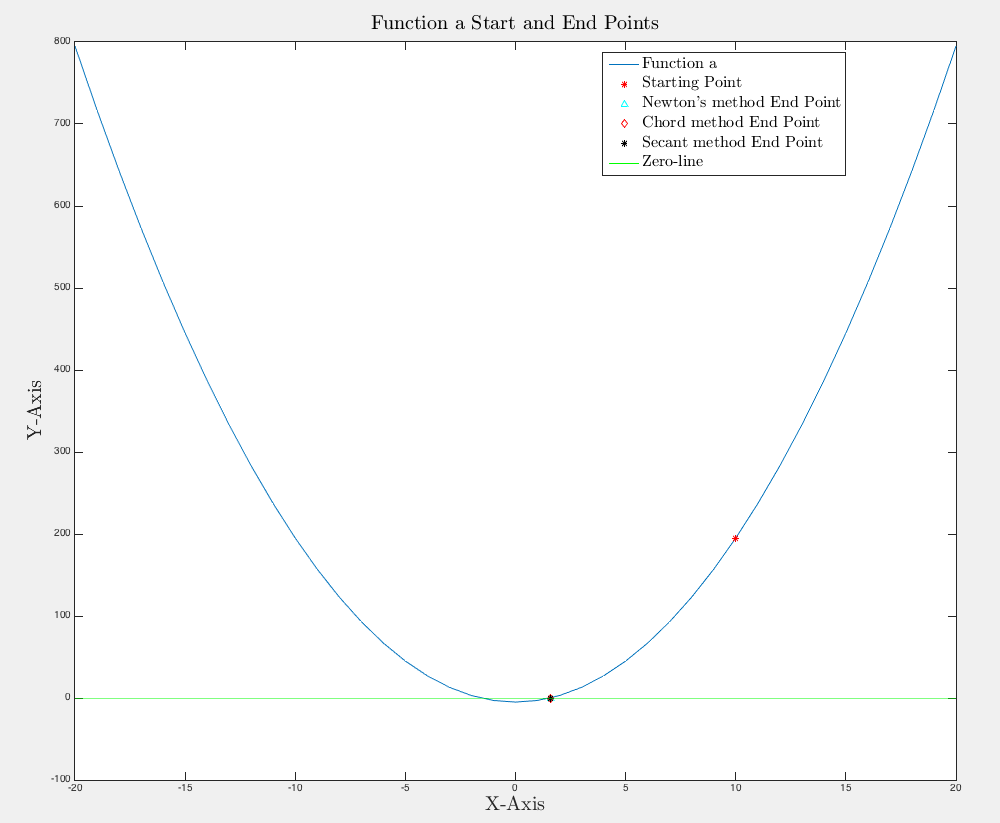
\includegraphics[width=140mm]{f1.png}
\caption{Initial conditions and final answer of Newton's Method, the Chord Method, and the Secant Method for Function a.}
\label{f1}
\end{center}
\end{figure}
\FloatBarrier

For Function b, once again, all three methods converged to the same point, as seen in Figure \ref{f2}. As can be seen in Figure \ref{count}, Newton's method once again converges the fastest, but is only marginally quicker than the other two methods. For both Functions a and b, the starting point was close enough to the $F(x^*)=0$ point that the methods were able to converge.

\begin{figure}[!h]
\begin{center}
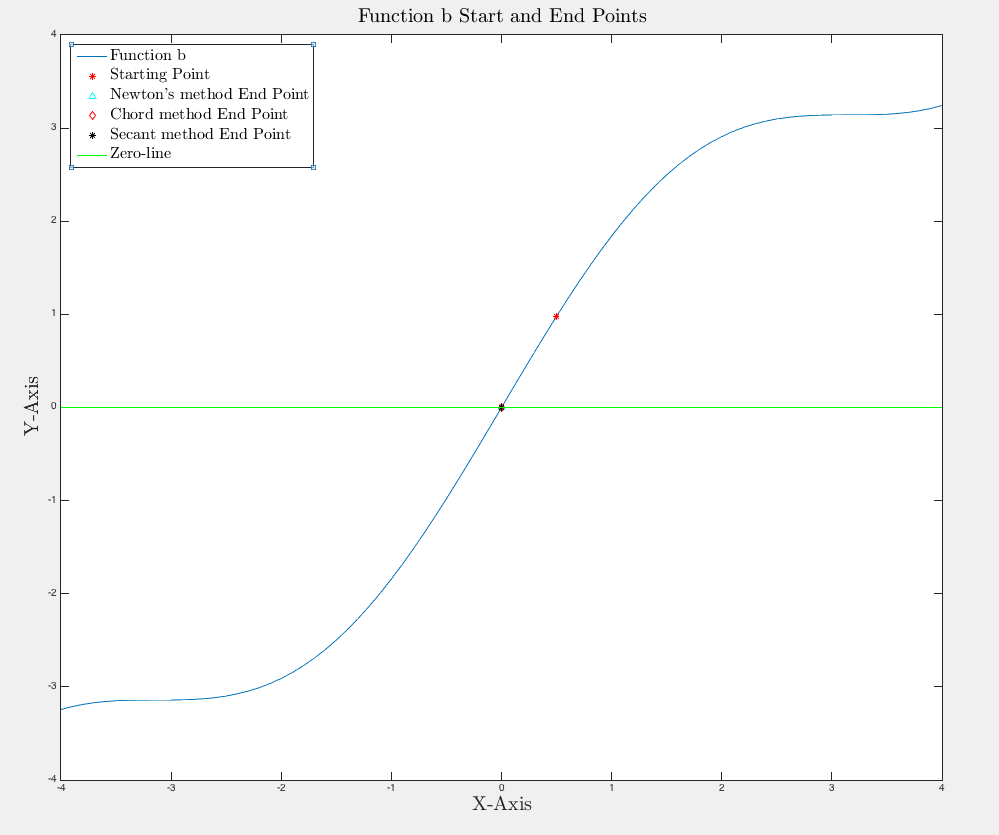
\includegraphics[width=140mm]{f2.png}
\caption{Initial conditions and final answer of Newton's Method, the Chord Method, and the Secant Method for Function b.}
\label{f2}
\end{center}
\end{figure}
\FloatBarrier
\begin{figure}[!h]
\begin{center}
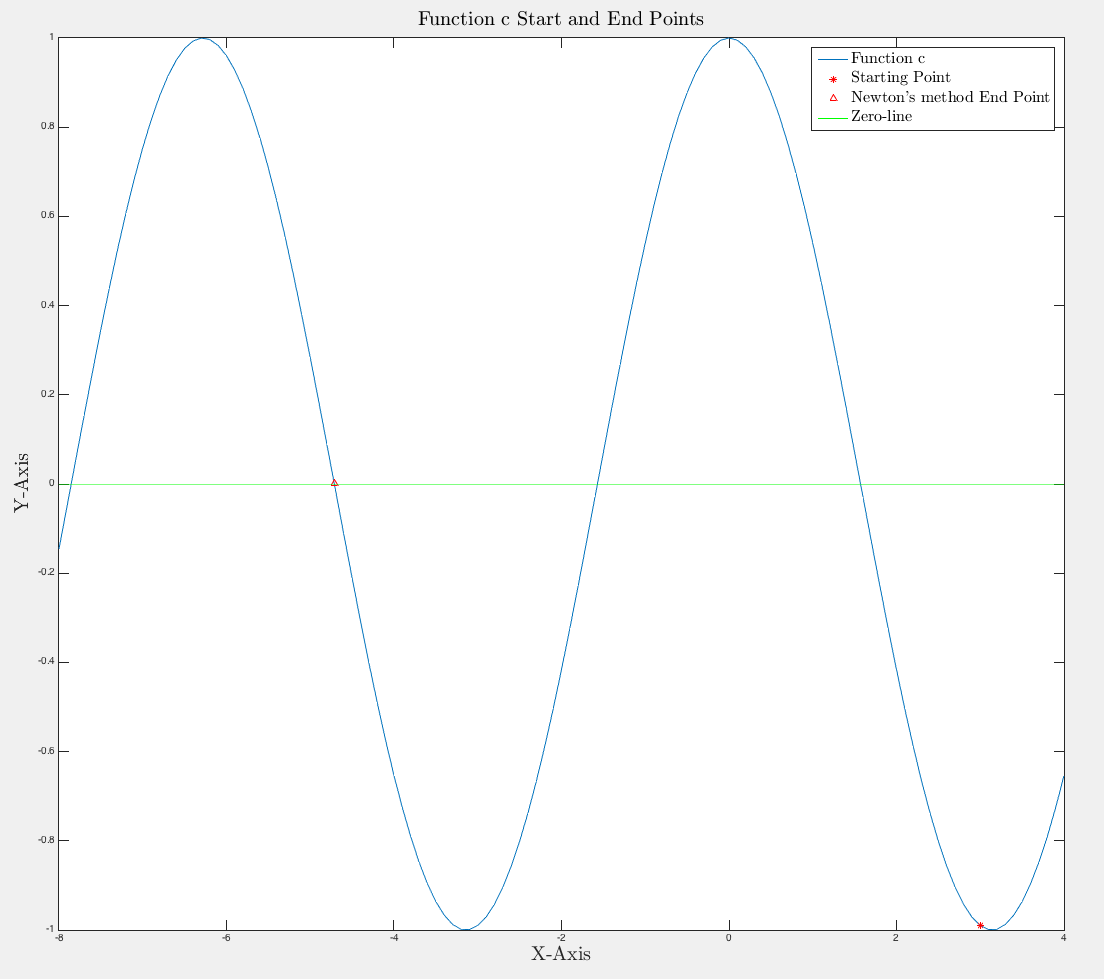
\includegraphics[width=140mm]{f3.png}
\caption{Initial conditions and final answer of Newton's Method, the Chord Method, and the Secant Method for Function c.}
\label{f3}
\end{center}
\end{figure}

 The Chord and Secant methods both had issues converging on Function c due to its periodic motion, as can be seen in Figures \ref{xvals},\ref{count}, and \ref{f3}. While Newton's method did find a point where $F(x)=0$, this was by no means the closest zero point. The Secant method diverged the fastest from the true solution, quickly reaching an x value equal to the computational precision of Matlab, which is $2^53$. At this point, the method is still working, but Matlab is unable to correctly calculate the next step. When $a_n$ is being calculated, a divide-by-0 error occurs and the program exits. The Secant method works by approximating the derivative, $F'(x)$ by using the previous step's $x$ and $F(x)$ values. However, with a periodic function, errors in the derivative can and will send the function off in an incorrect direction. If any $x$ point is closest to to an extreme on the y-axis, the Secant --- and Chord Method for that matter --- will go careening off into the distance. This doesn't mean that they won't eventually converge, but if they do it will be at a $F(x)=0$ far from the start point.
\FloatBarrier





%%%%%%%%%%%%%%%%%%%%%%%%%%%%%%%%%%%%%%%%%%%%%%%%%%%%%%%%
\section*{Question 3}
{\it Assume that the standard assumptions hold, that the cost of a function evaluation is \bigo($N^2$) floating-point operations, the cost of a Jacobian is \bigo($N$) function evaluations, and that $x_0$ is near enough to $x$ so that the Newton iteration converges quadratically to $x$. Estimate what is the number of iteration needed to obtain $||e_n||\le\epsilon||e_0||$, where $\epsilon$ is a small tolerance value. What is the number of floating point operations required to get this accuracy?}\newline


Newton's Method converges quadratically to $x$ and the error of the function is governed by the equation:
$$||\vec{x}_{n+1}-\vec{x}^*||\le k||\vec{x}_n-\vec{x}^*||^2
$$
where $\vec{x}^*$ is the solution, k is a constant, and $\vec{x}_n,\ \vec{x}_{n+1}$ are the values of $\vec{x}$ at steps $n$ and $n+1$. Since $\vec{x}^*$ is the solution, $\vec{x}_n-\vec{x}^*$ can be written as:
$$||\vec{e}_{n+1}||\le k||\vec{e}_{n}||^2\le(k||\vec{e}_{n-1}||^2)^2\le\dots
$$
We know from these equations and the problem statement that the Newton iteration converges quadratically and that the norm of the error is dependent upon the previous step's error. Thus, to get to $\vec{x}_n$, the error has converged by $
(k||\vec{x}_0-\vec{x}^*||^{2})^{n+1}=||\vec{e}_n||$. The number of iterations necessary to get to the $\epsilon$ tolerance is:
$$\frac{||\vec{e}_n||}{||\vec{e}_0||}=(k||\vec{x}_0-\vec{x}^*||^2)^{n}=\epsilon
$$
$$n=\frac{log(\epsilon)}{log(k||\vec{e}_0||^2)}
$$


Assuming that evaluating the function, $F(x)$ costs \bigo($N^2$) FLOPS and evaluating the Jacobian is only \bigo($N$) FLOPS, the number of of FLOPS required to get to an accuracy of $ \epsilon$ can be calculated. The breakdown of the FLOPS cost per step for Newton's method is given below:
\begin{align*}
\vec{r}&=||F(\vec{x})|| &\ \ \ \ N^2\ FLOPS\\
F_x&=\vec{r} & N\ FLOPS\ for\ an\ assignment\\
While\ ||F_x||&>\tau_r\vec{r}+\tau_a &\ \ \ n\ iterations\\
J&=F'(\vec{x}) &\ \ N\ FLOPS\\
\vec{s}&=-F(\vec{x})(F'(\vec{x}))^{-1} &Depends\ on\ how\ \vec{s}\ is\ solved.\ See\ Below\\
\vec{x}&=\vec{x}+\vec{s}&\ \ \ \ N\ FLOPS\\
F_x& =F(\vec{x}) & N^2\ FLOPS\\
end\\
\end{align*}
The cost per iteration for Newton's method is highly dependent upon how $\vec{s}$ is solved. From Homework 1, we know that the Conjugate Gradient method requires $\approx$ \bigo($160N$) FLOPS to reduce the error of the solver by a factor of $10^{-3}$. This value will be used as a rough estimate for the remained of this problem. Thus, adding up all of the FLOPS, it requires \bigo($N^2$) FLOPS to set up the problem, and \bigo($N^2+162N$) FLOPS per $n$ iterations. To get to the $\epsilon$ accuracy, it would take \bigo($(\frac{log(\epsilon)}{log(k||\vec{e}_0||^2)})(N^2+162N)+N^2$) FLOPS.

%%%%%%%%%%%%%%%%%%%%%%%%%%%%%%%%%%%%%%%%%%%%%%%%%%%%%%%%
\section*{Question 4}
{\it Answer the questions in the previous problem for the chord method.}\newline
Much of the previous problem's analysis carries over for this problem. One of the main differences between the Chord method and Newton's method is the Chord method converges at a linear rate in the area local to the solution. Because of this, the error equation presented in Problem 3 above changes to:
$$\frac{||\vec{e}_n||}{||\vec{e}_0||}=\frac{k||\vec{e}_0||||\vec{e}_n||}{k||\vec{e}_0||}=(||\vec{x}_0-\vec{x}^*||)^{n}=\epsilon
$$
$$n=\frac{log(\epsilon)}{log(k||\vec{e}_0||)}
$$
Because the Chord method is linear, the quadratic term in the  denominator changes into a linear term. Assuming that evaluating the function, $F(x)$ costs \bigo($N^2$) FLOPS and evaluating the Jacobian is only \bigo($N$) FLOPS, the number of of FLOPS required to get to an accuracy of $ \epsilon$ can be calculated. The breakdown of the FLOPS cost per step for the Chord method is given below:
\begin{align*}
\vec{r}&=||F(\vec{x})|| &\ \ \ \ N^2\ FLOPS\\
F_x&=\vec{r} & N\ FLOPS\ for\ an\ assignment\\
J&=F'(\vec{x}) &\ \ N\ FLOPS\\
L,U\ decomposition&\ of\ J& \ \frac{N^3}{3}\ FLOPS\ for\ Cholesky\ factorization\\
While\ ||F_x||&>\tau_r\vec{r}+\tau_a &\ \ \ n\ iterations\\
L\vec{y}&=-F(\vec{x}) &Forward\ Substitution\ N^2\ FLOPS\\
U\vec{s}&=\vec{y} &\ Back\ Substitution\ N^2\ FLOPS\\
\vec{x}&=\vec{x}+\vec{s}&\ \ \ \ N\ FLOPS\\
F_x& =F(\vec{x}) & N^2\ FLOPS\\
end\\
\end{align*}
Once again, the cost per iteration is dependent on how $\vec{s}$ is solved. Because the $L,U$ decomposition has been calculated prior to the start of the iteration section, the cost is only incurred once. While \bigo($\frac{N^3}{3}$) is the worst-case for decomposing the Jacobian, in reality, this value is dependent on the sparsity of the matrix. If the Jacobian is very sparse, the cost for decomposing it will be much smaller. Inside the iteration section, the $\vec{s}$ was solved using forward and backward substitution, but they could be easily calculated using two sequential Conjugate Gradient calls. 

The total cost of using the Chord method with Cholesky factorization of the Jacobian and Forward/Backward substitution is \bigo$((\frac{N^3}{3} +N^2 +2N)+(\frac{log(\epsilon)}{log(k||\vec{e}_0||)})(3N^2+N))$ FLOPS. This method, compared to Newton's method, has the potential for costing significantly more FLOPS to converge to a solution. However, if the Jacobian is extremely costly to evaluate, the Chord method has the advantage of only evaluating it once. 
%%%%%%%%%%%%%%%%%%%%%%%%%%%%%%%%%%%%%%%%%%%%%%%%%%%%%%%%
%\section*{Question 5}
%{\it Discreteize the following differential equation:
%$$\begin{cases} -u'' +4u = & x\in [0,1] \\ u(0)=-1, & u(1)=2 \end{cases}
%$$
%
%by the central difference scheme. Write your linear system of equations (you must give the matrix A and $\vec{b}$). Solve the system by using classical iteration such as Jacobi, Gauss-Seidel and SOR with n = 1000. Test you relaxation parameter in SOR for several values and decide which one is better. You need to discuss your results.}\newline
%
%The above differential equation can be solved analytically to generate a truth curve, against which the numerical methods can be compared. The solution for this particular ODE is:
%$$u(x)=\frac{e^{-2x}(e^{4x}+2e^{4x+2}-2e^2-e^4)}{e^4-1}
%$$
%
%To solve this equation numerically, the equation must first be discretized via the central difference theorem. The first step is to discretize the term $-u''$:
%$$u''=\frac{d^2u}{dx^2}=\frac{1}{h}\Bigg(\frac{u(x+h)-u(x)}{h}-\frac{u(x)-u(x-h)}{h}\Bigg) = \frac{1}{h^2}\bigg(u(x+h)-2u(x)+u(x-h)\bigg)
%$$
%
%This gives the final form of the differential equation, with the same boundary conditions, of:
%$$0=-\frac{1}{h^2}\bigg(u(x+h)-2u(x)+u(x-h)\bigg)+4u(x)
%$$
%Realizing that $h=x_i-x_{i-1}$, this can be simplified and rewritten as:
%$$0=u_{i+1}-2u_i+u_{i-1}-4h^2u_i
%$$
%
%This form of the equation can be used to generate the A and $\vec{b}$ variables, where $A\vec{u}=\vec{b}$:
%
%{\begin{center}
%$A= \begin{bmatrix}
%-2-4h^2 & 1 &0 &0 &0&\dots&0          \\[0.3em]
%1 &-2-4h^2 & 1 &0 &0&\dots&0     \\[0.3em]
%0 &1 &-2-4h^2 & 1 &0 &\dots&0 \\[0.3em]
%&&\ddots &\ddots &\ddots \\[0.3em]
%0&\dots&\dots&\dots&\dots&1&-2-4h^2 
%     \end{bmatrix}
%  $  ,  $\vec{u} = \begin{bmatrix}
%u_1          \\[0.3em]
%u_2\\[0.3em]
%\vdots \\[0.3em]
%u_{n-2}\\[0.3em]
%u_{n-1}
%     \end{bmatrix}
%  $  ,  $\vec{b}= \begin{bmatrix}
%1          \\[0.3em]
%0 \\[0.3em]
%\vdots\\[0.3em]
%0\\[0.3em]
%-2
%     \end{bmatrix}
%  $ 
%  \end{center}
%where $h=\frac{1}{n}$. This discretized ODE was then solved using the Gauss-Jacobi , Gauss-Seidel, and SOR with $n=1000$. 
%
%The A matrix as well as the b and u vectors were created with the following code:
%\lstinputlisting{SetupProb5.m}
%The first algorithm tested was the Gauss-Jacobi method. This is the simplest algorithm to implement and has a simple iteration. The G-J method is computed by the equation: 
%$$x_i^{(k+1)}=\frac{1}{a_{ii}}\bigg(b_i+\sum\limits_{\substack{j=1\\ j\ne i}}^n a_{ij}x_j^{(k)}\bigg) \ \ \ \ \ \ \ \ i=1:n
%$$
%The G-J algorithm can quickly be implemented in just a few lines in Matlab, using Matlab's vector notation. The implementation used for this problem is shown below.
%\lstinputlisting{Jacobi.m}
%The G-J method was run with a number of different convergence criteria to demonstrate the convergence properties of this method. Figure \ref{gj} shows these convergence values. The convergence criteria is defined as $|\vec{x}^{\ (k+1)}-\vec{x}^{\ (k)}|$. When the method is no longer making any significant changes to the $\vec{x}$ values, it has been deemed converged. This is used throughout this homework question as a metric for performance. 
%
%\begin{figure}[!h]
%\begin{center}
%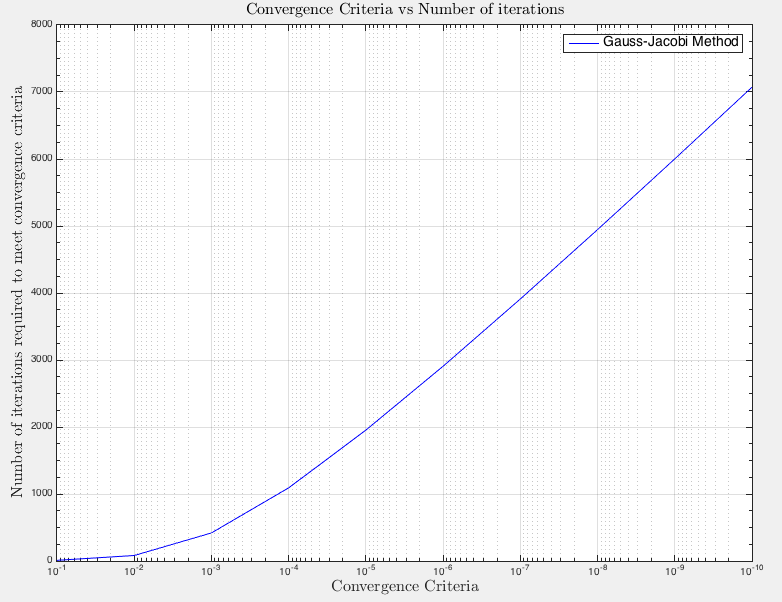
\includegraphics[width=130mm]{gj.png}
%\caption{Convergence of the G-J method.}
%\label{gj}
%\end{center}
%\end{figure}
%
%The Gauss-Jacobi method was used to check for the solution of the ODE. The solutions presented in Figure \ref{sol} show that as the maximum error decreases, the solution approaches that of the analytical solution, which is a straight line from -1 to 2. All of the numerical methods were checked to ensure the correct solutions were generated. 
%
%\begin{figure}[b!]
%\begin{center}
%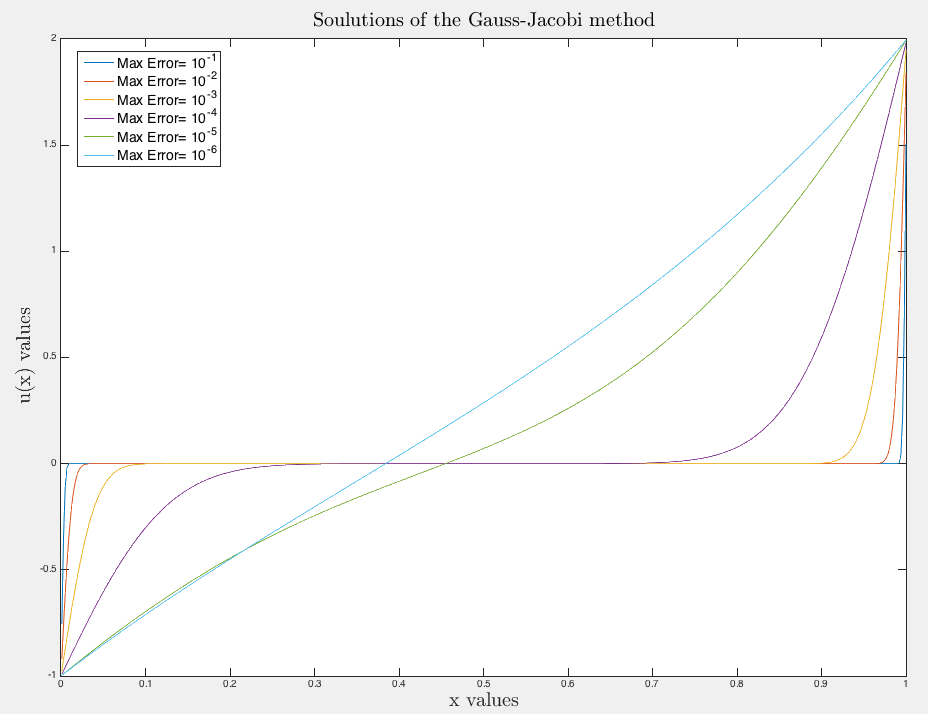
\includegraphics[width=135mm]{GJsol.png}
%\caption{The solutions of the G-J method. As the error decreases, the solution approaches a straight line.}
%\label{sol}
%\end{center}
%\end{figure}
%
%The second algorithm implemented was the Gauss-Seidel method. The G-S method splits the A matrix into the D, E, and F subparts. The D matrix contains all of the diagonal elements of A. The E and F matrices are the upper and lower triangular matrices, respectively, of A. The G-S algorithm then computes the following iteration:
%$$ \vec{x}^{\ (k+1)}=(D-E)^{-1}F\vec{x}^{\ (k)}+(D-F)^{-1}\vec{b}
%$$
%The G-S algorithm can also be quite quickly implemented in just a few lines in Matlab, using Matlab's vector notation. Notably, precomputing the values of $(D-E)^{-1}F$ and $(D-F)^{-1}\vec{b}$ greatly speedup the runtime of the algorithm, as these values are invariant. The implementation used for this problem is shown below.
%\lstinputlisting{GS.m}
%
%The G-S method was run with a number of different convergence criteria to demonstrate the convergence properties of this method. Figure \ref{sor} shows these convergence values. The chart also compares the relative performance of the G-J and G-S methods. As can be seen, for this particular case, the G-J and G-S methods seem to perform equally well. 
%
%The final method that was implemented was the Selective Over Relaxation (SOR) method. The SOR method is a variant of the Gauss-Seidel method that uses a relaxation parameter, $\omega$, to converge on the solution more efficiently. If $\omega=0.98$, this method behaves exactly the same as the Gauss-Seidel method. In fact, the code to generate the SOR method is nearly identical to that of the G-S method, except for the addition of computational line and one exit condition:
%
%\lstinputlisting{SOR.m}
%
%As can be seen in the SOR code, the value \mcode{xgs} is actually the output of the G-S method. This value is then modified by $\omega$ and blended with $(1-\omega)x_0$. The choice of the $\omega$ parameter is critical for this method to work effectively.  For this particular problem, $\omega$ values greater than 1.55 would result in the algorithm taking orders of magnitude longer to converge than the G-J or G-S methods. Thus, an additional exit condition was added to ensure the method would eventually cease. The optimal value of $\omega$ is defined as:
%$$ \omega_{opt}=\frac{2}{1+\sqrt{1-\rho(B)^2}}
%$$
%where $B=D^{-1}(E+F)$ and $\rho(B)$ is the spectral radius of $B$. For this discretized ODE, this value sits at $\approx 0.98$. The effect of the $\omega$ on the convergence of the SOR method can be seen in Figure \ref{omega}. In this plot, 34 different values of $\omega$ were used in the SOR calculation to determine the number of iterations necessary to converge to a solution. The 34 points are not equally spaced in this plot, but rather, there are more points near the minima value of $\omega=0.98$ to determine the actual best point. At an $\omega$ value of 1, the SOR method effectively becomes the G-S method, and thus the number of iterations required to converge spikes at 1. Due to the nature of the this particular ODE, values of $\omega$ greater than 1 were shown to be unstable. This is because the spectral radius of the B matrix, where $B=D^{-1}(E+F)$, was equal to 1. This means $\omega$ values larger than 1 will cause the system to become unstable and the x values will tend towards infinity. Thus, for Figure \ref{omega}, $\omega$ values were only plotted to from .1 to 1. 
%
%\begin{figure}[!h]
%\begin{center}
%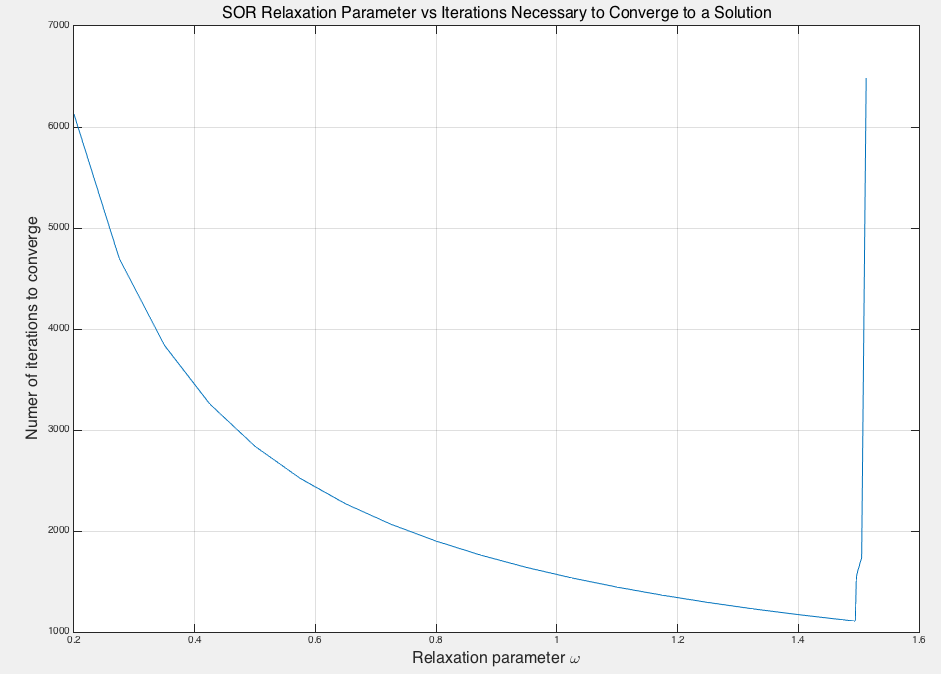
\includegraphics[width=140mm]{omega.png}
%\caption{Number of iterations necessary to converge to $10^{-6}$ vs $\omega$. The effects of $\omega$ on runtime can clearly be seen. }
%\label{omega}
%\end{center}
%\end{figure}
%
%\begin{figure}[!h]
%\begin{center}
%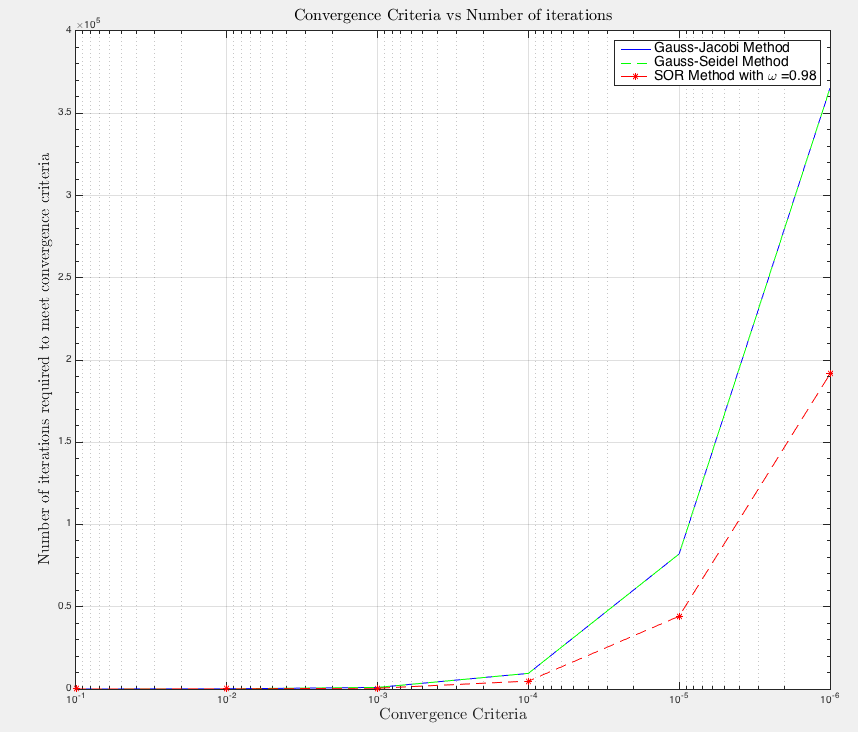
\includegraphics[width=140mm]{sor.png}
%\caption{SOR method vs G-S and G-J. }
%\label{sor}
%\end{center}
%\end{figure}
%
%Using the optimal value of $\omega=0.98$, the SOR method was compared to the G-S and G-J methods, as seen in Figure \ref{sor}. The SOR method is able to converge to a given solution in fewer iterations than either the G-J or G-S methods, due completely to the relaxation parameter. 
%
%
%
%


%\begin{figure}[htbp]
%\begin{center}
%\begin{tabular}{ | l | c|c| c| c | c | c| c| c| c  | c | }
%\hline
%  &A & B & C &D &E&F&G&H&I&J\ \\\hline
%  Design1 &240 & 350 & 305 & 30 & 35& 400& 90& 0& 30& 300 \\\hline
%% Design2 &300 & 380 & 370 & 34 & 40& 400& 100& 50& 100& 100 \\\hline
%%  Design3 &300 & 600 & 580 & 40 & 50& 550& 100& 150& 200& 250 \\\hline
%
%\end{tabular}
%\caption{Design 1 Parameters}
%\end{center}
%\end{figure}
%
%The isometric view of this design can be seen in Figure \ref{d1i}. The large cylinder was plotted using multiple instances of the \mcode{surf} command on two cylinders. Figure \ref{d1y} and Figure \ref{d1z} show the printer design in the X-Y and X-Z plains, respectively.
%
%\begin{figure}[htbp]
%\begin{center}
%\includegraphics[width=160mm]{d1iso.png}
%\caption{An isometric view of Design 1}
%\label{d1i}
%\end{center}
%\end{figure}

\FloatBarrier
\newpage
\appendix
\section*{Appendix A: Matlab code}
\subsection*{AutoRun}
\lstinputlisting{AutoRun.m}
\subsection*{Newton's Method}
\lstinputlisting{Newton.m}
\subsection*{Chord Method}
\lstinputlisting{Chord.m}

\subsection*{Secant Method}
\lstinputlisting{secant.m}


\end{document}  